\chapter{Sprint 1}
\label{chap:sprint1}
The development sprints are the most important parts of the scrum development process.
Therefore the sprint reports are a vital part of our final report of the project. The
following chapter presents an overview of how we planned, worked and completed Sprint 1.

Sprint 1 started on 5th of September and ended on 16th of September.
We had not yet decided on how long each sprint should be, and chose a duration of 11 days 
for Sprint 1. The reason behind this was high chance of changes in the applications.

The chapter is divided into five parts, starting with the overall plan for the sprint
in Section \ref{sec:sprint1plan}. Followed by the sprint backlog in Section 
\ref{sec:sprint1backlog}, which lists up the tasks that have been chosen for the sprint. 
Section \ref{sec:sprint1designAndImpl} will focus on the work made to the GUI, the logic 
implemented in the applications and the work done to the database. The chapter ends with 
what have been tested and the corresponding results in Section 
\ref{sec:sprint1testingAndResults} and a sprint review in Section \ref{sec:sprint1review}.

\section{Sprint Plan}
\label{sec:sprint1plan}
The plan for Sprint 1 was to set up the project, get the main screen up and running and
make screens for the distraction, without any animations. Finishes to the preliminary
studies were also to be made. We chose such a huge widespread of tasks from the backlog, since we wanted a skeleton of the application up and running.
Some connections between the different elements of the application were to be implemented,
but mainly we focused on the user interface. During the sprint we mainly did manual
testing, since there were not many changes to logical elements.

\section{Sprint backlog}
\label{sec:sprint1backlog}
The table \ref{sec:Sprint1Table} shows the sprint backlog for sprint 1, which is a smaller part of the
Product Backlog. The goal is to implement all tasks assigned to that sprint, and in this manner implement all task in the product backlog.

\begin{table}[t]
	\begin{center}
		\begin{tabular}{|c|p{0.3\linewidth}|l|l|l|}
			\hline
			\# ID & Task & Story points & Estimated hours & Responsible \\
			\hline
			1.1 & Add navigation between activities in main menu, for GAPP & 0.5 & 5 & Esben \\
			\hline
			1.2 & Add element for showing current medication plan & 0.5 & 5 & \\
			\hline
			1.3 & Add navigation between activities in main menu, for CAPP & 0.5 & 5 & Aleksander \\
			\hline
			1.4 & Make GUI for menu screen in GAPP & 2 & 20 & Jørgen \\
			\hline
			1.5 & Make GUI for menu screen in CAPP & 1.5 & 15 & Aleksander\\
			\hline
			1.6 & Add the adult app as a project to the repository & 0.5 & 5 & Yngve \\
			\hline
			2.1 & Make a screen for starting the treatment & 0.5 & 5 & Eirik \\
			\hline
			2.2 & Make a screen for finished treatment & 0.5 & 5 & Eirik \\
			\hline
			2.3 & Make a screen for distraction & 1 & 10 & Eirik \\
			\hline
			2.4 & Make some kind of distraction through the Karotz & 3 & 30 & \\
			\hline
			2.5 & Make a method for saving a treatment to the database & 3 & 30 & \\
			\hline
			2.6 & Make a method for starting treatment through Karotz & 1 & 10 & \\
			\hline
			2.7 & Make the database for saving treatments, medicine and avatar & 10 & 100 & Yngve \\
			\hline
			\bfseries{SUM} & & \bfseries{24.5} & \bfseries{245} & \\
			\hline
			\hline
		\end{tabular}
		\caption{Backlog for sprint 1}
		\label{sec:Sprint1Table}
	\end{center}
\end{table}

We also decided to continously write on the report, attend lectures and
hold advisor and customer meetings during the sprints. These are not included
in the backlog.

\section{Design and Implementation}
\label{sec:sprint1designAndImpl}
This section contains a description of the changes done in the respective areas of the development.

In Sprint 1 the main focus was to get the project up and running in Eclipse
and learning more about how Android works and getting used to Git. After a customer meeting in the middle of
the sprint, we had to change focus for a short period of time, since the customer
wanted to see more documentation and planning. After delivering a more concrete plan for the development, risk assesments and other important documents, we went back to programming.

We focused on working on smaller parts of the system at the time, rather than
starting too broad. This way we may deliver a working system, with some
functionality, rather than a system with much not-completely working functionality.
During this sprint the only feedback on the user interface was from the customers.

\subsection{User Interface Layer}
Before the sprint we had done one user testing on a paper prototype. The results were
used as an inspiration for the GUI for the time being. The project had earlier been divided
into two applications, one meant for children, CAPP (Child APPlication) and one meant for
adults, GAPP (Guardian APPlication). GAPP should consist of a log, a settings menu, an
information menu and an instruction option for treatment. CAPP should have a menu for the
avatar, a shop for buying stuff for the avatar and an instruction option for treatment.

We focused on the GUI of the main menu and navigating between different options, in both seperate
applications.

\subsection{Application Logic Layer}
There wasn't done any changes to the applications logic layers. The focus of the
sprint was mainly on GUI and the database.

\subsection{Data Persistence Layer}
%%%%%%%%%%%%%%%%%%%%%%%%%%%%%%%%%%%%%%%%%%%%%%%
%Reference to ER diagram :)
During the sprint, the database was created according to the existing specifications. Based
on an ER diagram that detailed the structure of tables in the database, it was implemented
in MySQL on NTNU's MySQL server.

During the sprint it was discussed wether the database should include internal procedures
for adding, updating and removing data. The alternative would be to rely in direct MySQL
queries. The advantage of using internal database procedures is that the access procedures
and the database itself are strongly related so keeping them separated would cause 
the system to be more distributed unnecessary, and therefore more difficult to maintain. 
The advantage of keeping the access in a separate layer, or programming each SQL query 
directly in the applications is that it would possibly save developer resources since it
is easier to write direct MySQL queries than processes. This question was still left
undecided at the end of sprint 1.

\section{Testing and Results}
\label{sec:sprint1testingAndResults}
This sections presents the testing done during the sprint and the results of the tests done.

\subsection{Testing}
During this early sprint our amount of testing was limited to two simple tests, where we tested
that the graphical user interface acted the way we desired it to, for both CAPP
and GAPP, respectively.

\begin{table}
	\begin{center}
		\begin{tabular}{|p{3.0cm}|p{14.0cm}|}
			\hline
			\bf{Item} & \bf{Description}\\
			\hline
			\bf{ID} & UNIT1.1\\
			\bf{Description} & Test of GUI for GAPP\\
			\bf{Date} & 17.09.2012\\
			\bf{Responsible} & Esben\\
			\bf{Subject} & The MainMenu class in the no.blopp.app.activity project.\\
			\bf{Precondition} & Early version of the application, runable on the android virtual device.\\
			\bf{Steps} & For each button on the MainMenu:\\
			\bf{} &
			\begin{tabulenum}
			\item Press the button.
			\item Confirm that you are moved to the appropriate screen.
			\item return to the main menu.
			\end{tabulenum}\\
			\hline
			\bf{Results} & As expected all buttons on the MainMenu directed us to the correct screen\\
			\hline
		\end{tabular}
	\end{center}
	\caption{Unit test 1.1, GAPP GUI}
	\label{tab:unit1.1}
\end{table}

\begin{table}
	\begin{center}
		\begin{tabular}{|p{3.0cm}|p{14.0cm}|}
			\hline
			\bf{Item} & \bf{Description}\\
			\hline
			\bf{ID} & UNIT1.2\\
			\bf{Description} & Test of GUI for CAPP\\
			\bf{Date} & 17.09.2012\\
			\bf{Responsible} & Aleksander\\
			\bf{Subject} & The MainMenu class in the no.blopp.app.med.activity project\\
			\bf{Precondition} & Early version of the application, runable on the android virtual device\\
			\bf{Steps} & For each button on the MainMenu:\\
			\bf{} &
			\begin{tabulenum}
			\item Press the button.
			\item Confirm that you are moved to the appropriate screen.
			\item return to the main menu.
			\end{tabulenum}\\
			\hline
			\bf{Results} & As expected all buttons on the MainMenu directed us to the correct screen\\
			\hline
		\end{tabular}
	\end{center}
	\caption{Unit test 1.2, CAPP GUI}
	\label{tab:unit1.2}
\end{table}

\subsection{Results}
The work done in Sprint 1 resulted in a skeleton for both seperate applications. It was possible to navigate 

\section{Sprint Retrospective}
\label{sec:sprint1review}
This section contains an evaluation of the sprint. The evaluation is done mainly
 by the us, but feedback from the customers are added to the retrospect.

\subsection*{What went well?}
The project is up an running. The developers have learned a lot more about Android and Android programming.
The database is running, even though the database is not tested. The documentation for the database and the plan for the project is complete.

\subsection*{What shall we start doing?}
We should do more testing. Testing the database and the logic of the applications should be done as the code is written.
We have discussed having programming sessions with all developers present, and is something we should start doing.
The customers has asked for more involvement with the documentation and the progress of the development, these requests should be fulfilled during the following sprints.

\subsection*{What could have gone better?}
We team should involve the customer more on different parts of the development.
We should have had early sessions to learn Android together, rather than apart.
We team should start sending meeting invitations earlier. The invitations should be sent at least 24 hours in
advance of internal meetings, and expectedly 48 hours in advance. For external meetings,
we team should send meeting invitations 72 hours in advance.

\subsection*{What should we stop doing?}
Nothing went completely wrong during this sprint.

\subsection{Sprint Burndown Chart}
In this section, an overview over the sprint backlog and the time spent on each backlog task in
addition to the estimate from earlier. The tasks we haven't worked on are shown without a responsible
developer and without time spent. The amount of work estimated to fill this sprint was highly over
estimated, due to using a very high hour value per story point. The progression was
as expected despite a slow start due to extra needs of documentation from the customer. The use of new
technology and a new development methology did also affect the pace of the development. Advisor and
customer meetings were held as usual during this sprint.

\begin{figure}
	\begin{center}
		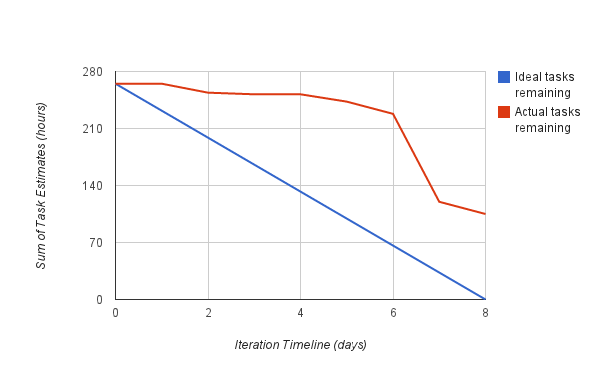
\includegraphics[width=15cm]{Pictures/Charts/Sprint1burndown}
	\end{center}
	\caption{Sprint 1 burndown chart}
	\label{fig:sprint1burndown}
\end{figure}

\begin{table}
	\centering
	\begin{sideways}
		\begin{tabular}{|c | p{4.8cm} | c | c | c | c | l |}
			\hline
			\# ID & Task & Story points & Estimated hours & Actual Hours & Time left & Responsible \\
			\hline
			1.1 & Add navigation between activities in main menu, for GAPP & 0.5 & 5 & 5 & 0 & Esben \\
			\hline
			1.2 & Add element for showing current medication plan & 0.5 & 5 & 0 & 5 & \\
			\hline
			1.3 & Add navigation between activities in main menu, for CAPP & 0.5 & 5 & 5.5 & 0 & Aleksander \\
			\hline
			1.4 & Make GUI for menu screen in GAPP & 2 & 20 & 3 & 10 & Jørgen \\
			\hline
			1.5 & Make GUI for menu screen in CAPP & 1.5 & 15 & 3.5 & 0 & Aleksander\\
			\hline
			1.6 & Add GAPP as a project to the repository & 0.5 & 5 & 1 & 0 & Yngve \\
			\hline
			2.1 & Make a screen for starting the treatment & 0.5 & 5 & 6 & 0 & Eirik \\
			\hline
			2.2 & Make a screen for finished treatment & 0.5 & 5 & 6 & 0 & Eirik \\
			\hline
			2.3 & Make a screen for distraction & 1 & 10 & 6 & 0 & Eirik \\
			\hline
			2.4 & Make some kind of distraction through the Karotz & 3 & 30 & 0 & 30 & \\
			\hline
			2.5 & Make a method for saving a treatment to the database & 3 & 30 & 0 & 30 & \\
			\hline
			2.6 & Make a method for starting treatment through Karotz & 1 & 10 & 0 & 30 & \\
			\hline
			2.7 & Make the database for saving treatments, medicine and avatar & 10 & 100 & 15 & 0 & Yngve \\
			\hline
			\bfseries{SUM} & & \bfseries{24.5} & \bfseries{245} & \bfseries{51} & \bfseries{105} & \\
			\hline
			\hline
		\end{tabular}
	\end{sideways}
	\caption{Sprint 1 burndown chart}
	\label{tab:sprint1burndown}
\end{table}

Table \ref{fig:sprint1burndown} and table \ref{tab:sprint1burndown} show the burndown chart from this sprint. A burndown chart is a
helpful tool for reflecting upon what have been done and also give a better
overview to how the work was done. The burndown chart from this sprint looks
bad at first, but then turns out better. The reason to the slow progress
was that we were told to work on documentation and other tasks not in the
sprint backlog. 

Our base goal is to finish 175 estimated work hours during each sprint, which with a base multiplier of 10
corresponds to $175/10=17.5$ story points. Even though only 51 work hours were documented in the sprint, 
there are also 105 work hours not done. This means that out of the total $24.5$ story points planned 
for the sprint, there are $105/10=10.5$ story points left. In other words, we completed $24.5-10.5=14$ of 
the planned story points, which is only $17.5-14=3.5$ less than our goal. This is a fairly good result.
The result for the dramatic decline in storypoints left midways is due to one
task being overestimated. We have learned from this, and believe we will
make better estimations in the future.